\subsection{Planificación de la capacitación}
A continuación se detallarán las capacitaciones que se brindarán a los dos grandes grupos de usuarios que posee YesDoc; ``usuario'' e ``Instituciones médicas que no posean un sistema'', aquellas instituciones médicas que posean un sistema implementado se les dará las pautas en el apartado de ``Implementación del sistema'' para que a través de la interfaz que ellos usen actualmente puedan consumir los recurso de la API.

\subsubsection{Capacitación e instrucciones de uso para los usuarios}
\paragraph{Objetivos}
Facilitar el uso de la aplicación y brindarle al usuario apoyo en us aprendizaje.
\paragraph{Destinatarios}
Médicos y usuarios interesados por su salud que quieran gestionar sus datos médicos a través de la plataforma, tenemos en cuenta que muchas de estas personas pueden no estar familiarizadas con el sistema.
\paragraph{Métodos de capacitación}

Se grabarán videos que expliquen y ejemplifiquen el funcionamiento del sistema, tanto desde el punto de vista del paciente como del médico.
Dichos videos se alojarán en \textit{YouTube}, y se publicarán en la página oficial de \textit{YesDoc}, dentro de la sección de ayuda y asistencia.

Se añadirán mensajes de ayuda sobre la interfaz del sitio web de \textit{YesDoc}, lo que permitirá explicar al usuario todas y cada una de las opciones existentes en la misma.
Esto se logrará mediante la integración de un asistente de iniciación interactiva que le permite, al usuario que ingresa por primera vez, conocer cuáles son las funcionalidades que brinda el sistema.
Además, se hará uso de la opción ``Ayuda'', que le permite al usuario poder encontrar rápidamente lo que está buscando y aprovechar al máximo cada una de las funcionalidades otorgadas.

El manual de usuario incluirá los siguientes apartados, y se desarrollará en la \textbf{Sección \ref{manual_usuario}}, ubicado en la \textbf{página \pageref{manual_usuario}}. % Mejor ponerlo en un ANEXO!!!
    \begin{itemize}
        \item   Portada.
        \item   Título.
        \item   Derechos de autor.
        \item   Prefacio: contiene detalles de los documentos relacionados y la información sobre cómo navegar por la guía del usuario.
        \item   Índice de contenido.
        \item   Guía de funciones: explica cómo utilizar las principales funciones del sistema, es decir, sus funciones básicas.
        \item   Solución de problemas: detalla los posibles errores o problemas que pueden surgir, junto con la forma de solucionarlos.
        \item   Preguntas frecuentes.
        \item   Dónde encontrar más ayuda, y datos de contacto.
        \item   Glosario de términos. %y, para documentos más grandes, un Índice.

    \end{itemize}
    
\subsubsection{Capacitación e instrucciones de uso para las instituciones}

A continuación se describirán todas las actividades que se llevarán a cabo para implementar el nuevo sistema en instituciones médicas. Se identificará a todas las personas responsables de cada actividad  y el tiempo correspondiente a cada una. 

Esta capacitación se realizará en aquellas instituciones que no posean un sistema previo y que quieran utilizar la interfaz otorgada por \textbf{\emph{YesDoc}}




\paragraph{Objetivos generales}
\begin{itemize}
	\item Preparar al personal para la ejecución eficiente de las responsabilidades que
	asuman en sus puestos.
	\item Brindar oportunidades de desarrollo personal en los cargos actuales y para
	otros puestos para los que el colaborador puede ser considerado.
	\item Modificar actitudes para contribuir a crear un clima de trabajo satisfactorio,
	incrementar la motivación del trabajador y hacerlo más receptivo a la
	supervisión y acciones de gestión
	\item Colaborar con política de calidad de la empresa de capacitación de personal
	en forma constante.
\end{itemize}

\paragraph{Objetivos específicos}
\begin{itemize}
	\item Proporcionar orientación e información relativa a los objetivos de sistema, funcionamiento, normas y políticas.
	\item Proveer conocimientos y desarrollar habilidades que cubran la totalidad de
	requerimientos para el desempleo de puestos específicos.
	\item  Actualizar y ampliar los conocimientos requeridos en áreas especializadas.
	\item Contribuir a elevar y mantener un buen nivel de eficiencia individual y
	rendimiento colectivo.
	\item  Ayudar en la preparación de personal calificado, acorde con los planes,
	objetivos y requerimientos de la Empresa.
	\item  Apoyar la continuidad y desarrollo institucional.
\end{itemize}

\paragraph{Metas}
Capacitar al personal para que sea capaz de utilizar de manera adecuada el sistema, explotando al máximo todas las funcionalidades ofrecidas y disminuyendo los tiempos de atención.


\paragraph{Destinatarios}
El Plan de Capacitación incluye al personal de la empresa como
\begin{itemize}
	\item Personal Administrativo.
	\item Personal Recepcionistas.
	\item Personal de atención telefónica.
	\item Personal técnico.
\end{itemize}


\paragraph{Requisitos y recursos para realizar el curso}
	El alumno debe tener conocimientos de uso y manejo de computadoras, este requisito es fundamental y creemos que las instituciones hacen cumplir este requisito a su personal.
	
	Las instituciones deben contar con un espacio físico para el dictado del curso, además es recomendable que cada dos personas haya una computadora.
	
\paragraph{Fines de la capacitación}
Se pretende capacitar al personal involucrado sobre el uso del sistema para que puedan realizar la carga fluida de los análisis a un  paciente específico.

El fin general es el de  lograr suavizar el cambio de plataforma, y de este modo lograr una adecuada adopción del sistema. Además ayuda a disminuir los errores por incomprensión de consignas básicas y ayuda a lograr un consenso de metodologías a llevar a cabo, disminuyendo la incertidumbre  sobre la acción a llevar a cabo al toparse ante casos comunes ya contemplados, a través de la capacitación constante e integradora del  proceso de desarrollo.

 

\paragraph{Plan de capacitación}
La \textbf{capacitación} es un proceso educacional de carácter estratégico aplicado de
manera organizada y sistemática, mediante el cual el personal adquiere o desarrolla
conocimientos y habilidades específicas relativas al trabajo, y modifica sus actitudes
frente a aspectos de la organización, el puesto o el ambiente laboral.

Para permitirle a las organizaciones de salud explotar las funcionalidades del sistema al máximo se realizarán capacitaciones al personal de salud que lo utilizará para de este modo asegurar de forma correcta la carga de los datos y garantizar el uso de la totalidad de las funcionalidades brindadas.



El recurso más importante en cualquier organización lo forma el personal implicado
en las actividades laborales. Por ello creemos importante y necesario la capacitación completa ya que  la conducta y rendimiento de los individuos influye
directamente en la calidad y optimización de los servicios que se brindan.



%En tal sentido se plantea, a continuación, el Plan de Capacitación Anual que ayudará al uso fluido y completo de la aplicación.
% !!!!!!!!!!!!!!!!!!!!!!!!!!!!!!!!!!!!!!!!!!!!!!!!!!!!!!!!!!!!!!!!!


\paragraph{Método de capacitación y evaluación}
    \begin{itemize}
    	\item \textbf{Curso de 3 semanas con dictado matutino: }El primer día se detalla la carga horaria restante, pero se pretende que la primer semana sea de 3 horas y las últimas dos de 2 horas.
        
Para el curso es necesario asistir con un pendrive, el cual se usará para compartir la documentación. Además se recomienda traer algún elemento para tomar notas (cuaderno, notebook, etc).

La capacitación se hará de a lotes de a pequeños lotes en las primeras horas de la mañana para evitar retrasos en el trabajo.
		\item \textbf{Presentación inicial: } Se expondrá a todo el público la filosofía de YesDoc y los objetivos que persigue para lograr, de este modo, un compromiso conjunto de todos los participantes de sistema.
        
	    \item \textbf{Presentación de “situaciones tipo”}: Instructor transmite por escrito y explica en
las capacitaciones, casos referentes a circunstancias que posiblemente se presentarán, además expone un caso en tiempo real de una situación no planificada. En estas exposiciones se pide a los participantes que tomen nota del caso para comprender el funcionamiento de modo general.

	    \item \textbf{Metodología de exposición - diálogo}: Se expondrá la guía de uso completa, para exponer todas las funcionalidades y para indicar punto por punto como utilizar el sistema.
        
% Charlas breves de media hora cada viernes de todo el personal presente en cada sucursal sobre sus experiencias aportando problemas, soluciones y actualizaciones.

% los primeros dos dias: observación y toma de apuntes
%Ellas sólo observaban el manejo dl sistema y tomaban apuntes d lo q yo hacia.. Se nos pidió q no interactuáramos tanto con ellas sino q fuera natural para q observaran una atención normal..Igual no se puede tenés q decirles algo jajaja

%En realidad lo q c pretendía es q ellas aprendieran nuestras técnicas d atención.. Uso d herramientas básicas (y m refiero al bloc d notas, cosas tontas q pueden acelerar las cosas).. Cortar pegar.. Pavadas básicamente..

%los siguientes dos dias: presentacion de este apunte como guia que fue en un proyector.. en esta etapa les agregaba info

%luego de eso ya era puesta en marcha del trabajo aprendido.. en donde las evaluaba observaba todo lo que hacian y las corregia.. (arreglaba todos los lios que se mandaban, jajajaja)
%luego de eso vinieron los examenes escritos
%y a esta altura ya no hay capacitacion pero si asesoramiento


	    \item \textbf{Revisión de evaluación de desempeño:} En los controles de evaluación de desempeño, se realizará un seguimiento del personal evaluándolos en el cumplimiento de sus actividades.
        
        Se harán observaciones individuales y el seguimiento se realizará de forma cercana para controlar y corregir situaciones.
        
%trabajos prácticos y actividades diarias registradas por el empleado para el seguimiento y estado de sus tareas.

    \end{itemize}
    
\clearpage
\subsubsection{Gantt}
En la \textbf{[Figura \ref{mu-tareas_capacitacion}]} se muestran las tareas necesarias para llevar a cabo la capacitación y en la \textbf{[Figura \ref{mu-gantt_capacitacion}]} el Diagrama de Gantt respectivo.

\begin{figure}
	\centering
	\includegraphics[width=1\textwidth]{img/tareas_capacitacion}
	\caption{Planificación de la capacitación}
	\label{mu-tareas_capacitacion}
\end{figure}


\begin{figure}
	\centering
	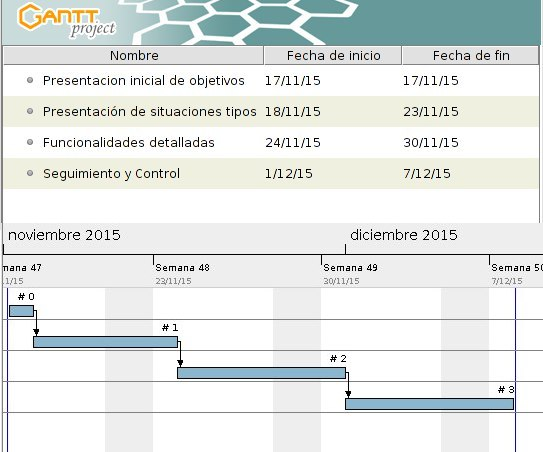
\includegraphics[width=15cm, height=5cm]{img/gantt_capacitacion}
	\caption{Gantt para la planificación de las capacitaciones}
	\label{mu-gantt_capacitacion}
\end{figure}

